\chapter{Resultados}\label{chap:resultados}

% AJUSTE: 12/10 — pedido do orientador: o capítulo passa a ser organizado por tipo de
% métrica (custo, qualidade, compromisso entre os dois), e cada tabela compara uma única
% grandeza. As tabelas são geradas por codigo/gerar_tabelas.py a partir dos CSVs. A
% terminologia "ingênua"/"guiada" passa a "sem"/"com análise de sensibilidade". Números do
% texto conferidos contra os CSVs: corrigidos as unidades de energia (eram µWh e mWh, o
% correto é mWh e Wh), a contagem de vitórias na magnitude (7 de 9, não 8 de 9), os fatores
% de ganho na estruturada (3 a 4 vezes só em 20--30%) e outras afirmações menores.
Este capítulo apresenta os resultados experimentais obtidos com o GPT-2
\textit{small} sobre o WikiText-2, organizados por tipo de métrica, de modo que cada
tabela compare uma única grandeza. Após o protocolo
(Seção~\ref{sec:res_protocolo}), a Seção~\ref{sec:res_custo} apresenta o custo
computacional e o consumo de energia das estratégias de poda, que respondem à primeira
pergunta do trabalho. A Seção~\ref{sec:perfil_sensibilidade} apresenta o perfil de
sensibilidade por camada, que alimenta a alocação com análise de sensibilidade, e a
Seção~\ref{sec:res_qualidade} compara a qualidade preditiva das alocações com e sem essa
análise, o que responde à segunda pergunta. A Seção~\ref{sec:res_finetune} submete as
configurações mais relevantes ao \textit{fine-tuning} de recuperação, a
Seção~\ref{sec:res_tradeoff} combina qualidade e energia nos indicadores da
Seção~\ref{sec:metodologia_metricas}, e a Seção~\ref{sec:res_sintese} sintetiza os
achados.

\section{Protocolo e Modelo de Referência}\label{sec:res_protocolo}

Todos os experimentos partem do GPT-2 \textit{small} pré-treinado
(124.439.808 parâmetros), avaliado no conjunto de teste do WikiText-2 por
janela deslizante com \textit{stride} de 512 \textit{tokens}. A perplexity do
modelo denso é de \textbf{25,17}. O valor é inferior aos 29,41 publicados por
\citeonline{Radford2019}, e a diferença é compatível com a do protocolo de
avaliação: com janelas deslizantes sobrepostas, cada \textit{token} é predito
com pelo menos 512 \textit{tokens} de contexto, o que reduz a
\textit{perplexity} em relação à avaliação em janelas disjuntas. A
documentação da biblioteca \texttt{transformers} registra esse efeito no
GPT-2 \textit{large}: 19,44 com janelas disjuntas de 1.024 \textit{tokens},
valor próximo dos 19,93 publicados, e 16,44 com \textit{stride} de 512
\cite{HuggingFacePerplexity}, redução de cerca de 15\%. Redução da mesma ordem,
cerca de 14\%, separa os 29,41 publicados para o \textit{small} dos 25,17
medidos aqui, com o mesmo protocolo daquela documentação. As medições de custo do modelo denso são: 474,70~MB
de memória de parâmetros e 126,6~GFLOPs por janela de 512 \textit{tokens}.

Duas ressalvas metodológicas condicionam a leitura das tabelas que se seguem.

A primeira é que \textbf{todos os resultados das varreduras são
\textit{one-shot}}, com exceção da Seção~\ref{sec:res_finetune}, dedicada
justamente ao retreinamento: poda-se o modelo pré-treinado e mede-se imediatamente, sem
qualquer \textit{fine-tuning} de recuperação. Essa escolha isola o efeito da
poda do efeito do retreinamento, mas implica que as perplexities aqui
reportadas são substancialmente piores que as da literatura, em que a poda é
seguida de retreinamento. As curvas não devem, portanto, ser lidas como
proposta de configuração de uso, e sim como medida do dano que cada estratégia
de alocação causa por si só. A Seção~\ref{sec:res_finetune} mostra que esse
dano é, em boa parte, reversível.

A segunda é que as varreduras foram executadas em sessões distintas do
ambiente Kaggle, e as medições de \textbf{custo dependem da sessão}. O mesmo
modelo denso registrou 40,5~ms por janela em uma sessão, 54,0~ms em outra e
46,3~ms em uma terceira; o consumo de energia do modelo denso variou de
forma análoga, entre 1176 e 1572~mWh por avaliação completa do conjunto de teste. Por
essa razão, a energia é sempre expressa pela redução relativa $\Delta E$
(Equação~\ref{eq:delta_e}), calculada em relação ao modelo denso medido na mesma sessão,
e nunca em valores absolutos; o tempo segue a mesma regra. As emissões de
$\text{CO}_2$, que dependem adicionalmente do fator de carbono da rede elétrica do
\textit{datacenter} --- que também variou entre sessões ---, não são comparadas entre
varreduras.

Os resumos por configuração (Seção~\ref{sec:metodologia_metricas}) usam as taxas de
10\% a 50\%. O corte em 50\% segue o critério daquela seção: até essa taxa, nenhuma
camada atinge o teto $r_{\max} = 0{,}95$ em nenhuma das alocações com análise de
sensibilidade, ao passo que a 60\% uma camada já o atinge na poda por magnitude e duas na
estruturada, com $\beta = 1{,}0$. O corte coincide com o ponto a partir do qual todas as
configurações estão inutilizáveis: a 60\%, a menor perplexity entre as oito avaliadas é de
1524,55, cerca de 61 vezes a do modelo denso. As taxas de 60\% a 90\% continuam reportadas
nas tabelas, mas não entram nas médias.

\section{Custo Computacional e Consumo de Energia}\label{sec:res_custo}

Esta seção responde à primeira pergunta do trabalho: em que medida a redução de
parâmetros se converte em redução real de custo. A Tabela~\ref{tab:custo} apresenta as
grandezas calculadas --- parâmetros, tamanho e FLOPs ---, e a Tabela~\ref{tab:energia}, a
grandeza medida: a redução relativa de energia.

\begin{table}[htb]
\centering
\caption{Custo calculado dos modelos podados, por taxa de poda. Na poda por magnitude,
os parâmetros são os não nulos, e os valores referem-se à alocação uniforme; a global
produz os mesmos valores, pois nenhuma das duas altera a arquitetura. Na poda
estruturada, a taxa de poda é a fração de estruturas removidas, e os valores referem-se à
alocação global; as demais alocações removem frações de parâmetros que diferem desta em
até 2,1 pontos percentuais.}
\label{tab:custo}
\small
% Gerado por codigo/gerar_tabelas.py a partir de codigo/resultados/. Não editar.
\begin{tabular}{c cc cc cc}
\toprule
& \multicolumn{2}{c}{\textbf{Parâmetros (M)}} & \multicolumn{2}{c}{\textbf{Tamanho (MB)}} & \multicolumn{2}{c}{\textbf{FLOPs (G)}} \\
\cmidrule(lr){2-3} \cmidrule(lr){4-5} \cmidrule(lr){6-7}
\textbf{Taxa de poda} & \textbf{Magn.} & \textbf{Estrut.} & \textbf{Magn.} & \textbf{Estrut.} & \textbf{Magn.} & \textbf{Estrut.} \\
\midrule
0\,\% & 124,4 & 124,4 & 474,7 & 474,7 & 126,6 & 126,6 \\
10\,\% & 115,9 & 116,0 & 474,7 & 442,6 & 126,6 & 118,0 \\
20\,\% & 107,5 & 107,6 & 474,7 & 410,5 & 126,6 & 109,3 \\
30\,\% & 99,0 & 99,0 & 474,7 & 377,6 & 126,6 & 100,5 \\
40\,\% & 90,5 & 90,6 & 474,7 & 345,5 & 126,6 & 91,9 \\
50\,\% & 82,0 & 81,9 & 474,7 & 312,6 & 126,6 & 83,1 \\
60\,\% & 73,5 & 73,5 & 474,7 & 280,5 & 126,6 & 74,5 \\
70\,\% & 65,0 & 65,1 & 474,7 & 248,3 & 126,6 & 65,9 \\
80\,\% & 56,5 & 56,5 & 474,7 & 215,5 & 126,6 & 57,0 \\
90\,\% & 48,0 & 48,1 & 474,7 & 183,3 & 126,6 & 48,4 \\
\bottomrule
\end{tabular}

\end{table}

\begin{table}[htb]
\centering
\caption{Redução relativa de energia $\Delta E$ (\%, Equação~\ref{eq:delta_e}) em relação
ao modelo denso medido na mesma sessão. Na poda por magnitude, os valores estão abaixo do
limiar de detecção do protocolo, de cerca de 10\%. $\beta$ é o expoente de intensidade da
Equação~\ref{eq:alocacao_dev}, que controla o quanto a alocação segue o perfil de
sensibilidade: com $\beta = 1{,}0$ o perfil é seguido integralmente, e com
$\beta = 0{,}5$ as diferenças entre camadas são atenuadas.}
\label{tab:energia}
\small
% Gerado por codigo/gerar_tabelas.py a partir de codigo/resultados/. Não editar.
\begin{tabular}{p{2.8cm} l rrrrrrrrr}
\toprule
& & \multicolumn{9}{c}{\textbf{Taxa de poda}} \\
\cmidrule(lr){3-11}
\textbf{Análise} & \textbf{Alocação} & 10\,\% & 20\,\% & 30\,\% & 40\,\% & 50\,\% & 60\,\% & 70\,\% & 80\,\% & 90\,\% \\
\midrule
\multicolumn{11}{l}{\textit{Poda não estruturada --- poda por magnitude}} \\
\multirow{2}{2.8cm}{Sem análise de sensibilidade} & Global & 1,7 & 2,6 & 2,8 & 3,7 & 4,1 & 5,3 & 6,2 & 7,7 & 9,0 \\
 & Uniforme & 2,1 & 3,0 & 2,4 & 3,1 & 4,4 & 5,0 & 5,9 & 7,4 & 8,9 \\
\multirow{2}{2.8cm}{Com análise de sensibilidade} & $\beta = 1{,}0$ & 3,8 & 3,8 & 3,9 & 4,7 & 5,8 & 5,8 & 6,4 & 6,9 & 6,8 \\
 & $\beta = 0{,}5$ & 3,5 & 3,5 & 3,8 & 4,3 & 5,0 & 5,6 & 6,3 & 6,9 & 7,1 \\
\midrule
\multicolumn{11}{l}{\textit{Poda estruturada --- cabeças de atenção e neurônios do MLP}} \\
\multirow{2}{2.8cm}{Sem análise de sensibilidade} & Global & 2,5 & 5,5 & 13,5 & 21,4 & 28,6 & 36,2 & 44,2 & 51,1 & 58,7 \\
 & Uniforme & 5,3 & 11,8 & 17,6 & 24,8 & 34,3 & 40,9 & 45,8 & 54,5 & 60,0 \\
\multirow{2}{2.8cm}{Com análise de sensibilidade} & $\beta = 1{,}0$ & 3,4 & 11,0 & 18,1 & 25,0 & 32,6 & 39,9 & 47,1 & 54,4 & 61,6 \\
 & $\beta = 0{,}5$ & 2,6 & 10,0 & 17,3 & 24,5 & 33,1 & 40,5 & 46,9 & 55,0 & 61,6 \\
\bottomrule
\end{tabular}

\end{table}

Na poda por magnitude, o resultado é negativo: \textbf{o custo não cai}. Entre 0\,\% e
90\,\%, o número de parâmetros não nulos cai de 124,4~M para 48,0~M --- uma redução de
61\,\% ---, enquanto o tamanho em memória e os FLOPs permanecem rigorosamente
constantes: 474,70~MB e 126,58~G em todas as dez taxas, valores idênticos dígito a
dígito. A explicação é direta: a poda não estruturada substitui pesos por zeros, mas não
remove nada da arquitetura. Os tensores mantêm as mesmas dimensões, e a GPU multiplica os
zeros exatamente como multiplicava os valores originais. O ganho de 61\,\% em parâmetros
é contábil, não físico.

As grandezas medidas comportam-se de modo ligeiramente diferente das calculadas:
$\Delta E$ cresce de forma pequena e monótona ao longo da varredura, até cerca de 9\,\% a
90\,\%, e o tempo de inferência cai 5,4\,\% entre os extremos (de 53,96 para 51,04~ms,
alocação uniforme). Essa deriva é da ordem da variação observada entre execuções do
mesmo modelo denso --- de 40,5 a 54,0~ms e de 1176 a 1572~mWh conforme a sessão
(Seção~\ref{sec:res_protocolo}) --- e não pode ser atribuída à poda, uma vez que a
arquitetura executada é a mesma em todas as taxas. Serve, na verdade, como calibração do
ruído de medição: qualquer efeito de poda inferior a cerca de 10\,\% em tempo ou energia
está abaixo do limiar de detecção deste protocolo. Na Tesla T4 utilizada, sem suporte de
\textit{hardware} ou de \textit{kernels} para esparsidade, a poda não estruturada não
entrega ganho de eficiência algum.

Na poda estruturada, ao contrário, \textbf{o custo cai, e cai proporcionalmente aos
parâmetros}: a 90\,\% de estruturas removidas, com a alocação global, o tamanho em
memória cai 61\,\%, os FLOPs 62\,\%, a energia 59\,\% e o tempo de inferência 56\,\%,
acompanhando a redução de 61\,\% no número de parâmetros. A redução de energia já supera o
limiar de detecção a 30\,\% (13,5\,\% na alocação global) e, a 90\,\%, é quase seis vezes
maior que ele. As duas estratégias formam, juntas, a resposta à primeira pergunta: a
redução de parâmetros só se converte em redução de consumo quando a poda remove
estruturas inteiras da arquitetura, e não quando apenas as zera.

As alocações com análise de sensibilidade preservam esse comportamento, o que era
esperado, uma vez que alteram a distribuição da poda, e não sua natureza. Na poda por
magnitude, $\Delta E$ permanece abaixo do limiar de detecção em todas as alocações. Na
poda estruturada, as quatro alocações têm $\Delta E$ próximo na mesma taxa: a 50\,\%,
28,6\,\% (global), 34,3\,\% (uniforme), 32,6\,\% ($\beta = 1{,}0$) e 33,1\,\%
($\beta = 0{,}5$). As diferenças, de até 6,3 pontos percentuais, são da ordem da variação
do próprio modelo denso dentro de um mesmo arquivo de resultados, que mediu 1,176~Wh na
série global e 1,261~Wh na uniforme, 7\,\% de diferença. A alocação global registra o menor
$\Delta E$ em todas as taxas, mas essa diferença não se separa da variação de medição, e
não é possível atribuir a nenhuma alocação vantagem de energia.

\section{Perfil de Sensibilidade por Camada}\label{sec:perfil_sensibilidade}

Antes da comparação de qualidade entre as alocações, esta seção apresenta o perfil de
sensibilidade que alimenta a alocação com análise de sensibilidade, levantado conforme a
Seção~\ref{subsec:fase1}: para cada uma das 12 camadas do GPT-2 \textit{small} e para cada
estratégia, poda-se \textbf{apenas} aquela camada à taxa-sonda, sem \textit{fine-tuning},
e a degradação $\Delta_{\ell}$ (Equação~\ref{eq:delta_perfil}) mede o aumento
logarítmico da perplexity em relação ao modelo denso. O levantamento foi feito a duas
taxas-sonda, 50\% e 30\%; as alocações usam apenas o perfil de 50\%, e o de 30\% serve de
verificação (Seção~\ref{subsec:robustez_sonda}).

\subsection{Perfil Obtido}\label{subsec:perfil_obtido}

A Tabela~\ref{tab:perfil_sensibilidade} apresenta os dois levantamentos, e a
Figura~\ref{fig:perfil_sensibilidade} representa graficamente o de 50\%.

\begin{table}[htb]
\centering
\caption{Perfil de sensibilidade por camada do GPT-2 \textit{small} no WikiText-2:
degradação $\Delta_{\ell}$ (Equação~\ref{eq:delta_perfil}) causada pela poda exclusiva da
camada indicada, sem \textit{fine-tuning}, a duas taxas-sonda. Entre parênteses, o posto
da camada na ordenação de sensibilidade (1 = mais sensível). As alocações usam apenas o
perfil de 50\,\%.}
\label{tab:perfil_sensibilidade}
\small
% Gerado por codigo/gerar_tabelas.py a partir de codigo/resultados/. Não editar.
\begin{tabular}{c cc cc}
\toprule
& \multicolumn{2}{c}{\textbf{Poda por magnitude}} & \multicolumn{2}{c}{\textbf{Poda estruturada}} \\
\cmidrule(lr){2-3} \cmidrule(lr){4-5}
\textbf{Camada} & \textbf{Sonda 30\,\%} & \textbf{Sonda 50\,\%} & \textbf{Sonda 30\,\%} & \textbf{Sonda 50\,\%} \\
\midrule
0 & 0,041 (1) & 0,390 (1) & 3,423 (1) & 4,009 (1) \\
1 & 0,007 (12) & 0,035 (12) & 0,159 (3) & 0,094 (11) \\
2 & 0,012 (7) & 0,093 (4) & 0,130 (7) & 0,173 (5) \\
3 & 0,007 (11) & 0,043 (11) & 0,143 (5) & 0,183 (4) \\
4 & 0,039 (2) & 0,202 (2) & 0,156 (4) & 0,218 (3) \\
5 & 0,035 (3) & 0,130 (3) & 0,093 (8) & 0,169 (6) \\
6 & 0,016 (4) & 0,074 (5) & 0,132 (6) & 0,138 (7) \\
7 & 0,008 (10) & 0,049 (10) & 0,053 (12) & 0,118 (10) \\
8 & 0,011 (8) & 0,055 (7) & 0,065 (10) & 0,122 (9) \\
9 & 0,014 (5) & 0,061 (6) & 0,060 (11) & 0,093 (12) \\
10 & 0,008 (9) & 0,054 (9) & 0,088 (9) & 0,138 (8) \\
11 & 0,013 (6) & 0,054 (8) & 0,539 (2) & 0,663 (2) \\
\midrule
\textbf{Razão máx./mín.} & 6,1$\times$ & 11,3$\times$ & 65,1$\times$ & 42,9$\times$ \\
\bottomrule
\end{tabular}

\end{table}

\begin{figure}[htb]
\centering
\caption{Degradação $\Delta_{\ell}$ causada pela poda isolada de cada camada,
à taxa-sonda de 50\,\%. Note-se que as escalas verticais diferem entre os dois
gráficos; na poda estruturada, a barra da camada 0 excede o eixo e está
truncada.}
\label{fig:perfil_sensibilidade}
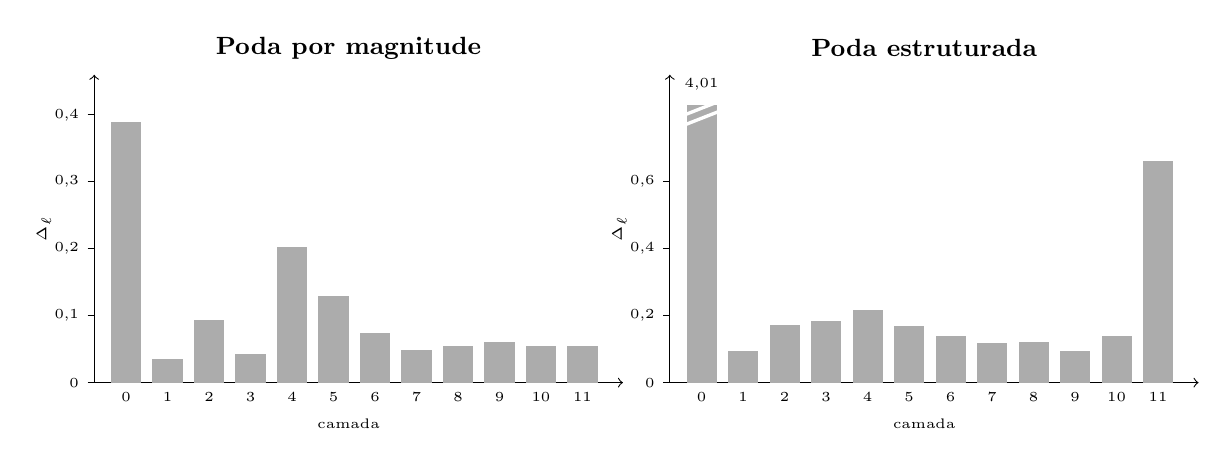
\begin{tikzpicture}[scale=0.85]

  % ---------- painel esquerdo: magnitude ----------
  \begin{scope}
    \draw[->] (-0.2,0) -- (7.7,0);
    \draw[->] (-0.2,0) -- (-0.2,4.6);
    \foreach \y/\lab in {0/0, 1/0{,}1, 2/0{,}2, 3/0{,}3, 4/0{,}4}
      \draw (-0.3,\y*1.0) -- (-0.2,\y*1.0) node[left,xshift=-2pt,font=\tiny] {\lab};
    \foreach \c/\d in {0/0.390, 1/0.035, 2/0.093, 3/0.043, 4/0.202, 5/0.130,
                       6/0.074, 7/0.049, 8/0.055, 9/0.061, 10/0.054, 11/0.054} {
      \fill[gray!65] ({\c*0.62+0.05},0) rectangle ++(0.45,{\d*10});
      \node[font=\tiny] at ({\c*0.62+0.275},-0.22) {\c};
    }
    \node[font=\small\bfseries] at (3.6,5.0) {Poda por magnitude};
    \node[font=\tiny] at (3.6,-0.62) {camada};
    \node[rotate=90,font=\tiny] at (-0.95,2.3) {$\Delta_{\ell}$};
  \end{scope}

  % ---------- painel direito: estruturada ----------
  \begin{scope}[xshift=8.6cm]
    \draw[->] (-0.2,0) -- (7.7,0);
    \draw[->] (-0.2,0) -- (-0.2,4.6);
    \foreach \y/\lab in {0/0, 1/0{,}2, 2/0{,}4, 3/0{,}6}
      \draw (-0.3,\y*1.0) -- (-0.2,\y*1.0) node[left,xshift=-2pt,font=\tiny] {\lab};
    \foreach \c/\d in {1/0.094, 2/0.173, 3/0.183, 4/0.218, 5/0.169,
                       6/0.138, 7/0.118, 8/0.122, 9/0.093, 10/0.138, 11/0.663} {
      \fill[gray!65] ({\c*0.62+0.05},0) rectangle ++(0.45,{\d*5});
      \node[font=\tiny] at ({\c*0.62+0.275},-0.22) {\c};
    }
    % camada 0: barra truncada
    \fill[gray!65] (0.05,0) rectangle (0.50,4.15);
    \draw[white,line width=1.2pt] (0.02,4.0) -- (0.53,4.2);
    \draw[white,line width=1.2pt] (0.02,3.85) -- (0.53,4.05);
    \node[font=\tiny] at (0.275,4.45) {4,01};
    \node[font=\tiny] at (0.275,-0.22) {0};
    \node[font=\small\bfseries] at (3.6,5.0) {Poda estruturada};
    \node[font=\tiny] at (3.6,-0.62) {camada};
    \node[rotate=90,font=\tiny] at (-0.95,2.3) {$\Delta_{\ell}$};
  \end{scope}

\end{tikzpicture}
\fonte{Elaborada pelo autor.}
\end{figure}

O primeiro resultado confirma a premissa da técnica: a sensibilidade está longe de ser
uniforme. Sob poda por magnitude, a camada mais frágil degrada o modelo 11,3 vezes mais
que a mais robusta; sob poda estruturada, 42,9 vezes mais, à taxa-sonda de 50\%. Tratar as
12 camadas como intercambiáveis --- que é exatamente o que a alocação uniforme faz ---
ignora uma diferença de uma ordem de grandeza no custo de podar cada uma delas.

\subsection{A Camada 0 como Gargalo}\label{subsec:camada_zero}

O segundo resultado é a magnitude do papel da primeira camada. Nas duas
estratégias ela é a mais sensível, mas o efeito é qualitativamente distinto no
caso estruturado: remover metade das cabeças de atenção e dos neurônios MLP
\textbf{apenas do bloco 0} eleva a perplexity de 25,17 para 1386,43, ou seja,
55 vezes o valor do modelo denso. Para dimensionar esse número, a poda
estruturada uniforme a 50\,\% --- que poda \textit{todas} as 12 camadas ---
atinge perplexity 4573,00. Em escala logarítmica, a camada 0 sozinha responde
por $4{,}01/5{,}20 \approx 77\,\%$ de toda a degradação produzida pela poda
uniforme do modelo inteiro.

A interpretação é coerente com o papel funcional do primeiro bloco. É nele que
as representações deixam de ser a soma direta de \textit{embeddings} de token
e de posição e passam a ser contextualizadas pela primeira vez; qualquer
informação descartada ali não tem como ser recuperada pelas camadas
subsequentes, que operam sobre um sinal já degradado. Trata-se, portanto, de
um erro que se propaga por toda a pilha, ao contrário de um erro cometido nas
camadas intermediárias.

Na poda estruturada observa-se ainda um segundo ponto crítico na outra
extremidade: a camada 11, imediatamente anterior à cabeça de linguagem,
apresenta $\Delta_{11} = 0{,}663$, quase cinco vezes a mediana das camadas
intermediárias. O perfil estruturado tem, assim, formato aproximado de ``U'':
as bordas da pilha são críticas e o miolo é comparativamente barato. Esse
padrão não se repete na poda por magnitude, cujo perfil decai após um pico
inicial e mantém as últimas camadas entre as mais robustas.

\subsection{Os Perfis Dependem da Estratégia}\label{subsec:perfis_divergem}

O terceiro resultado tem consequência metodológica direta: os dois perfis
\textbf{não} são o mesmo. A correlação de postos de Spearman entre eles é
$\rho = 0{,}50$ --- há concordância, mas parcial. As duas estratégias
coincidem em eleger a camada 0 como a mais crítica e em considerar as camadas
1 e 7 entre as mais robustas, e divergem em praticamente todo o resto: a
camada 11 é a segunda mais sensível sob poda estruturada e apenas a oitava sob
poda por magnitude; a camada 3 é a segunda mais robusta sob magnitude e a
quarta mais sensível sob poda estruturada.

A implicação prática é que não existe um perfil de sensibilidade único do
GPT-2. Sensibilidade é uma propriedade do par (camada, estratégia de poda),
não da camada isoladamente, e o perfil precisa ser levantado separadamente
para cada estratégia --- como foi feito aqui --- sob pena de se distribuir a
poda com um mapa que pertence a outro método. Esse achado também oferece
uma explicação para a inversão entre as alocações sem análise de sensibilidade
observada na Seção~\ref{sec:res_qualidade}: como magnitude de peso e norma de estrutura
respondem a aspectos diferentes da importância de uma camada, é esperado que a alocação
global (que decide com base nessas grandezas) acerte em um caso e erre no outro.

\subsection{Da Sensibilidade à Alocação}\label{subsec:alocacao}

O perfil é um diagnóstico; para virar estratégia, precisa ser convertido em
uma taxa de poda por camada. Essa conversão é a Equação~\ref{eq:alocacao_dev},
apresentada na Seção~\ref{subsec:fase2}: a taxa de cada camada é proporcional
à sua robustez --- o inverso da degradação medida --- elevada ao expoente
$\beta$, escalada por um fator único obtido por bisseção de modo que a
taxa de poda pretendida seja respeitada, e limitada pelo teto $r_{\max} = 0{,}95$.
Interessa aqui apenas o que ela produz na prática.

A Tabela~\ref{tab:alocacao_50} mostra as taxas que a
Equação~\ref{eq:alocacao_dev} produziu para uma taxa de poda de 50\,\% com
$\beta = 1$. O contraste com a alocação uniforme é acentuado: sob poda
estruturada, a camada 0 recebe 2\,\% de poda e a camada 1 recebe 84\,\%,
enquanto a alocação uniforme aplicaria 50\,\% a ambas.

\begin{table}[htb]
\centering
\caption{Taxas de poda por camada efetivamente aplicadas pela
Equação~\ref{eq:alocacao_dev} para taxa de poda de 50\,\% e $\beta = 1{,}0$
(coluna \texttt{taxas\_por\_camada} dos registros experimentais). $\beta$ é o expoente
de intensidade da equação, que controla o quanto a alocação segue o perfil de
sensibilidade; com $\beta = 1{,}0$, o perfil é seguido integralmente. A alocação
uniforme corresponderia a 50\,\% em todas as camadas.}
\label{tab:alocacao_50}
\small
% Gerado por codigo/gerar_tabelas.py a partir de codigo/resultados/. Não editar.
\begin{tabular}{l cccccccccccc}
\toprule
\textbf{Camada} & 0 & 1 & 2 & 3 & 4 & 5 & 6 & 7 & 8 & 9 & 10 & 11 \\
\midrule
Magnitude (\%) & 8 & 94 & 35 & 75 & 16 & 25 & 44 & 67 & 59 & 53 & 61 & 61 \\
Estruturada (\%) & 2 & 84 & 46 & 43 & 36 & 47 & 57 & 67 & 64 & 85 & 57 & 12 \\
\bottomrule
\end{tabular}

\end{table}

\subsection{Robustez do Perfil à Taxa-Sonda}\label{subsec:robustez_sonda}

O perfil que alimenta as alocações foi levantado a uma taxa-sonda de 50\,\%. Como a
escolha dessa taxa é arbitrária, cabe verificar se a ordenação de
sensibilidade que dela resulta é uma propriedade das camadas ou um artefato do
regime de poda em que a sonda opera. Para isso, o perfilamento completo foi
repetido a uma taxa-sonda de 30\,\%, nas duas estratégias, o que fornece uma
réplica independente da fase 1; a Tabela~\ref{tab:perfil_sensibilidade} traz os dois
levantamentos lado a lado.

A correlação de postos de Spearman entre as duas sondas é $\rho = 0{,}944$ na
poda por magnitude e $\rho = 0{,}713$ na poda estruturada. A ordenação é,
portanto, substancialmente estável --- e os achados que sustentam a estratégia
otimizada sobrevivem à troca de sonda. Na magnitude, as três camadas mais
sensíveis (0, 4 e 5) e as três mais robustas (1, 3 e 7) são \textbf{as mesmas}
nos dois levantamentos. Na estruturada, a camada 0 e a camada 11 ocupam os dois
primeiros postos em ambos, de modo que o formato em ``U'' discutido na
Seção~\ref{subsec:camada_zero} não depende da taxa-sonda; a camada 0 responde
por 65,5\,\% da soma dos $\Delta_{\ell}$ a 50\,\% e por 67,9\,\% a 30\,\%.

A estabilidade é menor na poda estruturada, e a divergência concentra-se em uma
camada: a camada 1 salta do 11º posto na sonda de 50\,\% para o 3º na de
30\,\%. A leitura mais plausível é que o miolo da pilha tem sensibilidades
próximas entre si --- os $\Delta_{\ell}$ das camadas 1 a 10 ficam todos entre
0,05 e 0,22 ---, de modo que pequenas variações de medição reordenam postos sem
alterar a estrutura do perfil. Isso é coerente com o comportamento do expoente
$\beta$ reportado na Seção~\ref{subsec:ablacao_beta}: o que a alocação
efetivamente aproveita é o sinal forte das bordas, não a ordenação fina do
miolo.

\subsection{Limitações do Perfilamento}\label{subsec:limitacoes_perfil}

Três limitações do procedimento devem ser explicitadas, pois condicionam a
leitura dos resultados da alocação com análise de sensibilidade.

A primeira é que, embora a verificação da seção anterior mostre que a
ordenação é estável entre 30\,\% e 50\,\%, ambas as taxas pertencem ao mesmo
regime intermediário de poda. Nada garante que a ordenação se mantenha em
regimes extremos --- poda muito branda, em que a degradação de todas as
camadas se aproxima do ruído de medição, ou muito agressiva, em que várias
camadas já colapsaram. Estender a verificação a essas faixas tem custo
proporcional: cada ponto de perfil exige uma avaliação completa de perplexity.

A segunda, e mais relevante, é que a sonda mede o efeito de cada camada
\textbf{isoladamente}, ignorando as interações entre elas. Os dados do próprio
experimento mostram que essa aproximação é imperfeita: a soma dos
$\Delta_{\ell}$ individuais sob poda por magnitude é 1,238, ao passo que a
poda uniforme simultânea de todas as camadas a 50\,\% produz degradação
logarítmica de 2,934 --- mais que o dobro. A degradação é fortemente
superaditiva, isto é, os erros introduzidos em camadas distintas se compõem em
vez de simplesmente se somarem. O perfil deve, por isso, ser lido como uma
ordenação relativa de importância, e não como um modelo preditivo da
degradação de uma configuração completa.

A terceira é que todas as medições são \textit{one-shot}, sem
\textit{fine-tuning} de recuperação. Camadas que parecem frágeis nesse regime
poderiam ser recuperáveis com retreinamento, o que eventualmente alteraria a
alocação ótima. A opção pelo regime \textit{one-shot} é deliberada e coerente
com o objetivo do trabalho --- isolar o efeito da poda do efeito do
retreinamento ---, mas restringe a generalidade das conclusões.

Nenhuma dessas limitações invalida o achado principal desta seção, que é
robusto às três: sob qualquer leitura, as camadas do GPT-2 diferem entre si
por mais de uma ordem de grandeza no custo de serem podadas, e essa diferença
é informação que as alocações uniforme e global simplesmente não utilizam. Se
essa informação se converte em ganho efetivo na fronteira entre compressão e
qualidade é o que a seção seguinte verifica.

\section{Qualidade Preditiva}\label{sec:res_qualidade}

Esta seção responde à segunda pergunta do trabalho: se a alocação com análise de
sensibilidade melhora o compromisso entre compressão e qualidade em relação às alocações
sem essa análise. As Tabelas~\ref{tab:comp_magnitude} e~\ref{tab:comp_estruturada}
apresentam a perplexity das quatro alocações em cada taxa de poda. A alocação com análise
de sensibilidade foi avaliada com dois valores do expoente $\beta$, 1,0 e 0,5, sobre o
mesmo perfil. Um terceiro valor, $\beta = 0$, não é uma alocação candidata, e sim um
controle: nele a regra atribui a mesma taxa a todas as camadas e deve reproduzir a
alocação uniforme (Seção~\ref{subsec:controle_beta_zero}).

\subsection{Poda por Magnitude}\label{subsec:aloc_magnitude}\label{sec:res_magnitude}

\begin{table}[htb]
\centering
\caption{Perplexity da poda por magnitude, sem retreinamento, nas quatro alocações. Em
negrito, o menor valor de cada taxa. $\beta$ é o expoente de intensidade da
Equação~\ref{eq:alocacao_dev}, que controla o quanto a alocação segue o perfil de
sensibilidade: com $\beta = 1{,}0$ o perfil é seguido integralmente, e com
$\beta = 0{,}5$ as diferenças entre camadas são atenuadas.}
\label{tab:comp_magnitude}
\small
% Gerado por codigo/gerar_tabelas.py a partir de codigo/resultados/. Não editar.
\begin{tabular}{c cc cc}
\toprule
& \multicolumn{2}{c}{\textbf{Sem análise de sensibilidade}} & \multicolumn{2}{c}{\textbf{Com análise de sensibilidade}} \\
\cmidrule(lr){2-3} \cmidrule(lr){4-5}
\textbf{Taxa de poda} & \textbf{Global} & \textbf{Uniforme} & $\boldsymbol{\beta = 1{,}0}$ & $\boldsymbol{\beta = 0{,}5}$ \\
\midrule
0\,\% & \multicolumn{4}{c}{25,17 (modelo base)} \\
10\,\% & \textbf{25,40} & 25,47 & 25,44 & 25,44 \\
20\,\% & 26,87 & 27,22 & 26,79 & \textbf{26,57} \\
30\,\% & 40,23 & 36,42 & 34,62 & \textbf{31,20} \\
40\,\% & 165,20 & 104,82 & 193,83 & \textbf{57,30} \\
50\,\% & 1096,50 & 473,28 & 1026,09 & \textbf{447,57} \\
60\,\% & 5121,25 & 2004,20 & \textbf{1524,55} & 2171,79 \\
70\,\% & 9371,16 & 6891,85 & \textbf{1853,30} & 2805,39 \\
80\,\% & 8847,27 & 10871,00 & \textbf{2747,56} & 3715,68 \\
90\,\% & \textbf{4612,69} & 13996,88 & 10398,10 & 7616,63 \\
\bottomrule
\end{tabular}

\end{table}

Nas alocações sem análise de sensibilidade, a curva de perplexity apresenta um joelho
acentuado em torno de 30\,\%. Até 20\,\% a poda é praticamente gratuita (acréscimo de 0,2
a 2,1 pontos de perplexity); a partir de 40\,\% a degradação torna-se explosiva. A região
utilizável em regime \textit{one-shot} é, portanto, limitada a taxas de até 20\,\%.

A comparação entre as duas alocações sem análise de sensibilidade revela um cruzamento
duplo: a global apresenta valores ligeiramente menores até 20\,\%, a uniforme domina
claramente entre 30\,\% e 70\,\% --- exatamente a faixa em que a escolha de alocação
teria consequência prática --- e a global volta a apresentar valores menores em 80\,\% e
90\,\%, região em que ambos os modelos já estão destruídos (perplexity acima de 4600) e a
comparação perde sentido. Na faixa que importa, portanto, a alocação uniforme é
preferível à global. Esse é um resultado contraintuitivo: a alocação global é a que
distribui a poda com base em uma medida de importância --- a magnitude do peso --- e
ainda assim perde para a alocação que ignora qualquer medida de importância. Trata-se do
primeiro indício de que a magnitude do peso é um \textit{proxy} pobre para a importância
de um parâmetro.

A alocação com análise de sensibilidade vence as duas em sete das nove taxas, de 20\,\%
a 80\,\%, e as margens são substanciais na faixa de interesse. Em 30\,\%, a perplexity
cai de 36,42 (melhor alocação sem análise de sensibilidade) para 31,20 --- uma redução de
14\,\%. Em 40\,\%, de 104,82 para 57,30, ou seja, a degradação é praticamente
\textbf{reduzida à metade} na mesma taxa de poda. Em 50\,\%, a vantagem persiste, ainda
que modesta (447,57 contra 473,28). De 60\,\% a 80\,\%, a configuração com
$\beta = 1{,}0$ produz perplexities de 1,3 a 3,7 vezes menores que a melhor alocação sem
análise de sensibilidade --- embora, nesse regime, todos os modelos já estejam degradados
a ponto de a comparação ter interesse mais teórico que prático. Na média geométrica de
10\,\% a 50\,\% (Seção~\ref{sec:metodologia_metricas}), a melhor configuração com análise
de sensibilidade ($\beta = 0{,}5$, 55,80) fica cerca de 15\,\% abaixo da melhor sem ela
(uniforme, 66,00).

As derrotas ocorrem nos extremos. Em 10\,\%, a alocação global (25,40) fica 0,04 abaixo
das duas configurações com análise de sensibilidade (25,44), diferença sem consequência
prática. Em 90\,\%, a global apresenta o menor valor, mas, como a perplexity de todas as
configurações ultrapassa 4600, a ordenação entre modelos igualmente inservíveis não
carrega significado.

\subsection{Poda Estruturada}\label{subsec:aloc_estruturada}\label{sec:res_estruturada}

\begin{table}[htb]
\centering
\caption{Perplexity da poda estruturada, sem retreinamento, nas quatro alocações; a taxa
de poda é a fração de estruturas removidas. Em negrito, o menor valor de cada taxa.
$\beta$ é o expoente de intensidade da Equação~\ref{eq:alocacao_dev}, que controla o
quanto a alocação segue o perfil de sensibilidade: com $\beta = 1{,}0$ o perfil é seguido
integralmente, e com $\beta = 0{,}5$ as diferenças entre camadas são atenuadas.}
\label{tab:comp_estruturada}
\small
% Gerado por codigo/gerar_tabelas.py a partir de codigo/resultados/. Não editar.
\begin{tabular}{c cc cc}
\toprule
& \multicolumn{2}{c}{\textbf{Sem análise de sensibilidade}} & \multicolumn{2}{c}{\textbf{Com análise de sensibilidade}} \\
\cmidrule(lr){2-3} \cmidrule(lr){4-5}
\textbf{Taxa de poda} & \textbf{Global} & \textbf{Uniforme} & $\boldsymbol{\beta = 1{,}0}$ & $\boldsymbol{\beta = 0{,}5}$ \\
\midrule
0\,\% & \multicolumn{4}{c}{25,17 (modelo base)} \\
10\,\% & 356,20 & 481,13 & \textbf{124,29} & 215,83 \\
20\,\% & 2102,06 & 1484,89 & \textbf{371,07} & 717,19 \\
30\,\% & 2413,52 & 5467,56 & \textbf{724,53} & 923,65 \\
40\,\% & 2434,92 & 10486,71 & \textbf{1301,15} & 9489,87 \\
50\,\% & 2402,58 & 4573,00 & \textbf{2327,59} & 7922,81 \\
60\,\% & \textbf{2957,26} & 5799,76 & 5393,15 & 12322,05 \\
70\,\% & \textbf{4635,36} & 12249,58 & 10130,33 & 103463,60 \\
80\,\% & \textbf{7620,02} & 53313,38 & 8891,77 & 203995,84 \\
90\,\% & 5822,89 & 827316,19 & 5353,85 & \textbf{4830,24} \\
\bottomrule
\end{tabular}

\end{table}

Na poda estruturada, o preço da redução de custo é severo em regime \textit{one-shot}. Já
com 10\,\% de estruturas removidas, a perplexity da alocação global salta de 25,17 para
356,20 --- compare-se com 25,40 na poda por magnitude à mesma taxa. \textbf{Não existe
região gratuita} na poda estruturada sem retreinamento, o que é coerente com o
procedimento original de \citeonline{Li2017}, em que a poda é sempre seguida de
\textit{fine-tuning}.

A inversão observada na magnitude repete-se ao contrário: entre as alocações sem análise
de sensibilidade, é a \textbf{global} que domina na poda estruturada, com exceção da taxa
de 20\,\%, e a uniforme colapsa em taxas altas (perplexity de 53.313 a 80\,\% e de 827.316
a 90\,\%, contra 7620 e 5823 da global). Somado ao resultado da poda por magnitude, isso
estabelece que \textbf{nenhuma das duas alocações sem análise de sensibilidade vence nas
duas estratégias} --- a constatação que motiva a análise de sensibilidade.

A comparação entre os dois tipos de estrutura acrescenta uma assimetria. Remover cabeças
de atenção é notavelmente mais tolerável que remover neurônios MLP: com 129 das 144
cabeças removidas (90\,\%), a perplexity fica em 781, ao passo que a remoção equivalente
de neurônios MLP produz valores acima de 3900. A curva das cabeças é, ainda, não
monotônica, com mínimo local em torno de 30\,\% (perplexity 162, inferior aos 237 obtidos
com apenas 10\,\% removidas) --- eco direto do achado de \citeonline{Michel2019} sobre a
redundância das cabeças de atenção. Em contrapartida, as camadas MLP concentram cerca de
dois terços dos parâmetros podáveis, de modo que a poda restrita a cabeças tem alcance
limitado como estratégia de compressão.

A alocação com análise de sensibilidade, com $\beta = 1{,}0$, obtém a menor perplexity em
todas as taxas de 10\,\% a 50\,\%. A vantagem é máxima entre 20\,\% e 30\,\%: em 20\,\%, a
perplexity cai de 1484,89 (melhor alocação sem análise de sensibilidade) para 371,07, um
fator de \textbf{quatro}; em 30\,\%, de 2413,52 para 724,53, um fator de 3,3. Em 10\,\%,
o fator é de 2,9 (356,20 contra 124,29). A partir daí, a vantagem diminui: o fator é de
1,9 em 40\,\% (2434,92 contra 1301,15), e a diferença é marginal em 50\,\% (2402,58 contra
2327,59). Na média geométrica de 10\,\% a 50\,\%, a perplexity cai de 1602,62 (global)
para 632,46, um fator de 2,5. Considerando que não existe região gratuita para a poda
estruturada \textit{one-shot}, reduzir a perplexity a um quarto na mesma taxa de poda é o
resultado mais expressivo deste capítulo.

Uma ressalva quantitativa é necessária. Como a remoção de estruturas é
discreta, as taxas fracionárias por camada não são atingíveis exatamente, e a
alocação com análise de sensibilidade acaba removendo uma fração de parâmetros
ligeiramente menor que a global no mesmo alvo: em 10\,\%, esparsidade real de 9,20\,\%
contra 9,90\,\%; em 30\,\%, 29,01\,\% contra 29,95\,\%. Parte da
vantagem observada deve-se, portanto, a um corte marginalmente menor. A
diferença é de menos de um ponto percentual de esparsidade, ao passo que a
diferença de perplexity chega a um fator de quatro, de modo que a explicação
não se sustenta como causa principal --- mas o efeito existe e deve ser
declarado.

De 60\,\% a 80\,\%, a ordenação se inverte e a alocação global volta a vencer; em
90\,\%, a perplexity de todas as configurações supera 4800, e a ordenação perde
significado. A causa da inversão é identificável nas taxas alocadas: a partir de 60\,\%,
um número crescente de camadas satura no teto $r_{\max} = 0{,}95$ --- duas camadas em
60\,\%, quatro em 70\,\%, oito em 80\,\% e onze em 90\,\%. Saturadas as
camadas, a alocação deixa de discriminar entre elas e degenera em algo próximo
da poda uniforme sobre o subconjunto saturado, ao mesmo tempo em que concentra
uma pressão crescente sobre as poucas camadas ainda livres. A alocação com análise de
sensibilidade, portanto, \textbf{só é informativa enquanto a taxa de poda couber dentro
do teto por camada}, o que justifica o corte das médias em 50\,\%
(Seção~\ref{sec:res_protocolo}). Esse é um limite intrínseco de qualquer alocação
proporcional com teto, e não um defeito de implementação.

\subsection{O Controle $\beta = 0$}\label{subsec:controle_beta_zero}

Antes de interpretar a ablação, cabe verificar se a regra de alocação está
correta. Com $\beta = 0$ o fator $\Delta_{\ell}^{-\beta}$ da
Equação~\ref{eq:alocacao_dev} vale 1 para toda camada, de modo que todas recebem
a mesma taxa e a alocação deve coincidir com a varredura uniforme
correspondente. É um teste de sanidade barato, pois reaproveita o perfil já
levantado.

Na poda estruturada a coincidência é \textbf{exata}: nas dez taxas de
poda, a alocação com $\beta = 0$ reproduz a perplexity da varredura
uniforme até a última casa decimal registrada --- 5467,5635 em 30\,\%,
4573,0020 em 50\,\% e 827.316,1875 em 90\,\%, para citar três níveis. A
identidade confirma que a conversão de perfil em taxas, a bisseção do fator de
escala e a aplicação das taxas por camada estão implementadas corretamente: o
que a alocação com análise de sensibilidade obtém a mais, nas seções anteriores, vem do
perfil, e não de alguma diferença espúria de procedimento.

Na poda por magnitude a coincidência \textbf{não} ocorre, e a razão é uma
diferença deliberada de implementação que merece registro. A varredura uniforme
decide um limiar de magnitude para cada matriz de peso isoladamente, ao passo
que a alocação por camada decide um limiar único por bloco, compartilhado pelas
quatro projeções que o compõem. As duas produzem a mesma esparsidade agregada
--- exatamente 30\,\%, 50\,\% e assim por diante ---, mas distribuída de
forma diferente entre as projeções de um mesmo bloco, e as perplexities
divergem: 473,28 contra 590,25 em 50\,\%, e 13.996,88 contra 8610,96 em
90\,\%. A alocação com $\beta = 0$ não é, portanto, a poda
uniforme da Seção~\ref{sec:res_magnitude}, e sim uma terceira alocação
--- ``global dentro da camada'' --- cuja comparação com as demais fica fora do
escopo deste trabalho. Para a poda estruturada, que é a estratégia
efetivamente capaz de reduzir consumo, o controle vale integralmente.

\subsection{Ablação do Expoente $\beta$}\label{subsec:ablacao_beta}

A comparação entre $\beta = 1{,}0$ e $\beta = 0{,}5$ produz um resultado que
não era antecipado: \textbf{o valor adequado de $\beta$ depende da
estratégia}, e depende dela de forma oposta nas duas.

Na poda estruturada, $\beta = 1$ domina em todos os níveis até 80\,\%, e o
amortecimento é francamente prejudicial --- em 70\,\% e 80\,\% a configuração
com $\beta = 0{,}5$ produz perplexities de 103.463 e 203.996, uma ordem de
grandeza pior que qualquer outra alocação testada. Na poda por magnitude ocorre
o inverso na faixa útil: $\beta = 0{,}5$ é melhor de 20\,\% a 50\,\%; de 60\,\% a 80\,\%
o expoente pleno passa à frente, e em 90\,\% $\beta = 0{,}5$ volta a ser melhor
(7616,63 contra 10398,10).

A explicação mais plausível liga-se à dispersão dos perfis. O perfil
estruturado tem razão máximo/mínimo de 42,9$\times$ e é dominado pela camada 0,
cuja fragilidade é tão extrema (Seção~\ref{subsec:camada_zero}) que qualquer
amortecimento da alocação lhe atribui uma taxa de poda maior, com consequências
catastróficas: em 70\,\%, $\beta = 0{,}5$ atribui 14,6\,\% de poda à camada 0,
contra 3,0\,\% de $\beta = 1$. Quando o perfil contém um sinal dessa
intensidade, convém segui-lo integralmente. Já o perfil de magnitude tem
dispersão de 11,3$\times$, distribuída entre várias camadas de sensibilidade
intermediária; nele, a razão entre camadas é mais suscetível a ruído de
medição, e amortecê-la funciona como regularização. O expoente $\beta$
comporta-se, assim, como um parâmetro de confiança no perfil: quanto mais
nítido o sinal, maior o $\beta$ que compensa adotar.

\section{\textit{Fine-tuning} de Recuperação}\label{sec:res_finetune}

% AJUSTE: 03/10 — "fecha a lacuna", expressão que o orientador marcou como confusa na
% Metodologia, reescrita aqui do mesmo modo que nos capítulos 4 e 5.
Todas as varreduras apresentadas até aqui operam em regime \textit{one-shot}.
Esta seção reporta a Etapa 4 (Seção~\ref{sec:finetuning}), que incorpora o
retreinamento ao experimento para medir quanto da degradação causada pela poda
pode ser recuperada: as sete configurações definidas na
Seção~\ref{subsec:ft_configuracoes} foram submetidas ao
\textit{fine-tuning} de recuperação, com a perplexity medida antes e depois do
retreinamento.
% AJUSTE: 03/10 — "orçamento" fica reservado ao orçamento de poda (definido na
% Metodologia); no sentido de treino, passa a "quantidade de retreinamento".
A quantidade de retreinamento é
idêntica para todas: uma época sobre o conjunto de treino do WikiText-2, 297
passos do otimizador, taxa de aprendizado de $5 \times 10^{-5}$ e semente
fixa. Diferentemente das demais, esta varredura foi executada integralmente
em uma única sessão, de modo que suas medições de tempo e energia são
diretamente comparáveis entre si.

\begin{table}[htb]
\centering
\caption{Perplexity antes (\textit{one-shot}) e depois do \textit{fine-tuning} de
recuperação (uma época, 297 passos). Sem análise de sensibilidade, a alocação é a uniforme
na poda por magnitude e a global na estruturada; com análise de sensibilidade, usa-se
$\beta = 1{,}0$, o expoente de intensidade da Equação~\ref{eq:alocacao_dev} com o qual a
alocação segue integralmente o perfil de sensibilidade. A razão expressa a perplexity
pós-retreinamento como múltiplo da do modelo denso retreinado, e não do modelo denso
original.}
\label{tab:finetune}
\small
% Gerado por codigo/gerar_tabelas.py a partir de codigo/resultados/. Não editar.
\begin{tabular}{l rrr rrr}
\toprule
& \multicolumn{3}{c}{\textbf{Sem análise de sensibilidade}} & \multicolumn{3}{c}{\textbf{Com análise de sensibilidade}} \\
\cmidrule(lr){2-4} \cmidrule(lr){5-7}
\textbf{Configuração} & \textbf{\textit{One-shot}} & \textbf{Pós-FT} & \textbf{Razão} & \textbf{\textit{One-shot}} & \textbf{Pós-FT} & \textbf{Razão} \\
\midrule
Denso (controle) & \multicolumn{6}{c}{25,17 \textit{one-shot}; 18,68 pós-FT (referência da razão)} \\
\midrule
Magnitude 30\,\% & 36,42 & 20,54 & 1,10 & --- & --- & --- \\
Magnitude 50\,\% & 473,28 & 30,27 & 1,62 & --- & --- & --- \\
Estruturada 10\,\% & 356,20 & 25,33 & 1,36 & 124,29 & 25,96 & 1,39 \\
Estruturada 30\,\% & 2413,52 & 104,78 & 5,61 & 724,53 & 56,08 & 3,00 \\
\bottomrule
\end{tabular}

\end{table}

\subsection{O Controle Denso Reenquadra a Leitura}\label{subsec:controle_denso}

O primeiro resultado da Tabela~\ref{tab:finetune} não envolve poda alguma: o
modelo denso, submetido à mesma quantidade de retreinamento, tem sua perplexity
reduzida de 25,17 para \textbf{18,68}. São 26\,\% de ganho obtidos sem
remover um único parâmetro, atribuíveis exclusivamente à adaptação de domínio
--- o GPT-2 foi pré-treinado no WebText, não no WikiText-2, e o retreinamento
o aproxima da distribuição da base de dados de avaliação.

A consequência metodológica é considerável e justifica retroativamente a
decisão de incluir o controle. Sem ele, a configuração de magnitude a
30\,\% pareceria ter \textit{superado} o modelo original: 20,54 contra 25,17,
uma leitura que sugeriria que a poda melhora o modelo. A comparação correta é
contra 18,68, e diante desse valor a mesma configuração aparece pelo que de
fato é --- 10\,\% pior que o denso equivalente. As colunas de razão da
Tabela~\ref{tab:finetune} adotam essa referência, a única leitura que
separa recuperação do dano da poda de mera adaptação à base de dados.

\subsection{A Recuperação é Substancial, mas Desigual}\label{subsec:recuperacao}

O retreinamento recupera uma fração expressiva do dano em todas as
configurações, e a magnitude dessa recuperação é inversamente proporcional à
qualidade do ponto de partida. A poda estruturada a 30\,\%, que o regime
\textit{one-shot} deixara em perplexity 2413,52 --- um modelo destruído para
qualquer propósito prático ---, retorna a 104,78. A poda por magnitude a
50\,\%, em 473,28, retorna a 30,27, isto é, a 1,62 vez o denso retreinado.

Esse comportamento qualifica de forma importante a leitura das seções
anteriores. A perplexity \textit{one-shot} mede o dano imediato da poda, mas
superestima o dano permanente: configurações que pareciam inutilizáveis são,
após uma quantidade modesta de retreinamento, recuperáveis a patamares
utilizáveis. A região praticável da poda, delimitada em 20\,\% de esparsidade
na Seção~\ref{sec:res_magnitude}, estende-se consideravelmente quando o
retreinamento é incluído.

Registre-se ainda que a hierarquia entre granularidades se mantém: a
configuração de magnitude a 30\,\% atinge a menor perplexity pós-retreinamento
de todas as configurações podadas (20,54), mas, pelas razões estabelecidas na
Seção~\ref{sec:res_custo}, não reduz tempo, energia nem memória. As
configurações estruturadas a 30\,\%, essas sim, registram 40,82~ms por janela e
1,285~Wh por avaliação completa contra 50,21~ms e 1,588~Wh do denso retreinado --- uma
redução de aproximadamente 19\,\% em ambos.

\subsection{O \textit{Fine-tuning} Corrói a Vantagem da Análise de
Sensibilidade}\label{subsec:ft_corroi}

O achado mais desconfortável desta varredura diz respeito diretamente à
contribuição central do trabalho. As linhas de poda estruturada da
Tabela~\ref{tab:finetune} confrontam, nas mesmas duas taxas de poda, a alocação global e a
alocação com análise de sensibilidade, antes e depois do retreinamento.

Em 10\,\% de estruturas removidas, a vantagem \textbf{desaparece}. Em regime
\textit{one-shot}, a alocação com análise de sensibilidade registrava perplexity 124,29
contra 356,20 da alocação global, uma vantagem de 2,87 vezes. Após o retreinamento, a
relação se inverte: 25,96 contra 25,33, com ligeira vantagem para a alocação
global. Em 30\,\%, a vantagem sobrevive, mas reduzida quase à metade: o fator
de 3,33 vezes do regime \textit{one-shot} (724,53 contra 2413,52) torna-se
1,87 vez (56,08 contra 104,78).

A interpretação é que a alocação com análise de sensibilidade otimiza uma quantidade
específica --- o dano imediato causado pela poda --- e o retreinamento repara
justamente o tipo de dano que ela evita. Quanto maior a quantidade de
retreinamento, menor a importância de haver podado bem. Sob essa leitura, o
perfil de sensibilidade é mais valioso quanto mais escassa for a quantidade de
retreinamento disponível, e a vantagem tende a crescer com a severidade da
poda, o que é consistente com sua persistência em 30\,\% e seu
desaparecimento em 10\,\%.

O achado não invalida a contribuição, mas delimita seu escopo com precisão: em
taxas de poda elevadas, a alocação com análise de sensibilidade continua entregando
perplexity aproximadamente duas vezes menor ao mesmo custo computacional
--- 40,28~ms e 1,307~Wh contra 40,82~ms e 1,285~Wh da alocação global em
30\,\%, valores equivalentes dentro da variação de medição. Em taxas de poda
baixas, seguidas de retreinamento, a alocação sem análise de sensibilidade é suficiente.

\subsection{Verificações de Integridade e Custo}\label{subsec:ft_verificacoes}

Duas verificações confirmam a correção do procedimento. A esparsidade das
configurações de magnitude, medida ao final do treinamento, permanece em
exatamente 30,0000\,\% e 50,0000\,\%, o que confirma que a máscara binária
descrita na Seção~\ref{sec:finetuning} foi corretamente reaplicada após cada
passo do otimizador e que o modelo não voltou a ser denso. As esparsidades
reais das configurações com análise de sensibilidade, por sua vez, ficam
ligeiramente abaixo do alvo (9,20\,\% e 29,01\,\% contra 9,90\,\% e 29,95\,\%
das configurações globais), diferença atribuível à granularidade discreta das
estruturas removidas --- uma cabeça de atenção ou um neurônio MLP são
indivisíveis. A diferença favorece marginalmente a alocação com análise de
sensibilidade e está registrada aqui por transparência, ainda que inferior a um ponto
percentual.

Quanto ao custo, o retreinamento consome 7,33~Wh no modelo denso, contra
1,59~Wh de uma avaliação completa do mesmo modelo --- aproximadamente 4,6
vezes. Trata-se, porém, de um custo pago uma única vez, ao passo que a
economia por inferência da poda estruturada se acumula a cada uso. A
configuração estruturada a 30\,\% economiza 0,303~Wh por avaliação completa
do conjunto de teste (1,285 contra 1,588~Wh), de modo que o custo do próprio
retreinamento se amortiza em aproximadamente 24 avaliações equivalentes --- um
volume trivial para um modelo em uso continuado. Cabe explicitar a unidade:
o consumo é medido em torno do bloco de avaliação inteiro, que percorre todo o
conjunto de teste por janela deslizante, e não em torno de uma janela
individual. Converter a economia para base por janela exigiria registrar o
número de janelas de cada avaliação, o que não foi feito; a amortização fica,
portanto, expressa na unidade efetivamente medida.

A limitação principal desta varredura é a quantidade de retreinamento: uma
única época. Não é possível afirmar, a partir destes dados, se a erosão da
vantagem da alocação com análise de sensibilidade se estabiliza no patamar observado em
30\,\% ou se prossegue com mais épocas até desaparecer também nessa taxa. Trata-se da
verificação mais imediata que este trabalho deixa em aberto.

\section{Compromisso entre Qualidade e Energia}\label{sec:res_tradeoff}

As seções anteriores trataram o custo e a qualidade separadamente. A
Tabela~\ref{tab:tradeoff} combina as duas grandezas nos indicadores da
Seção~\ref{sec:metodologia_metricas}.

\begin{table}[htb]
\centering
\caption{Indicadores de compromisso entre qualidade e energia
(Seção~\ref{sec:metodologia_metricas}). Sem retreinamento, cada configuração é resumida
pelas médias de 10\,\% a 50\,\% --- geométrica para a perplexity e aritmética para
$\Delta E$ ---, com $\eta$ calculado a partir delas; $S^*_E$ é a maior taxa com
perplexity até 5\,\% acima da do modelo denso (26,43). Após o \textit{fine-tuning}, os
valores são por configuração, e a referência é o modelo denso retreinado; nenhuma
configuração fica dentro do limite de 5\,\% (19,62). $\beta$ é o expoente de intensidade
da Equação~\ref{eq:alocacao_dev}, que controla o quanto a alocação segue o perfil de
sensibilidade.}
\label{tab:tradeoff}
\small
% Gerado por codigo/gerar_tabelas.py a partir de codigo/resultados/. Não editar.
\begin{tabular}{l r r r c}
\toprule
\textbf{Configuração} & \textbf{PPL} & $\boldsymbol{\Delta E}$ \textbf{(\%)} & $\boldsymbol{\eta}$ & $\boldsymbol{S^*_E}$ \\
\midrule
\multicolumn{5}{l}{\textbf{Sem retreinamento} (médias de 10\,\% a 50\,\%)} \\
Modelo base & 25,17 & 0,0 & 1,000 & --- \\
\multicolumn{5}{l}{\quad\textit{Poda por magnitude}} \\
\qquad Sem análise de sensibilidade --- global & 86,97 & 3,0 & 0,298 & 10\,\% \\
\qquad Sem análise de sensibilidade --- uniforme & 66,00 & 3,0 & 0,393 & 10\,\% \\
\qquad Com análise de sensibilidade --- $\beta = 1{,}0$ & 85,96 & 4,4 & 0,306 & 10\,\% \\
\qquad Com análise de sensibilidade --- $\beta = 0{,}5$ & 55,80 & 4,0 & 0,470 & 10\,\% \\
\multicolumn{5}{l}{\quad\textit{Poda estruturada}} \\
\qquad Sem análise de sensibilidade --- global & 1602,62 & 14,3 & 0,018 & --- \\
\qquad Sem análise de sensibilidade --- uniforme & 2847,86 & 18,7 & 0,011 & --- \\
\qquad Com análise de sensibilidade --- $\beta = 1{,}0$ & 632,46 & 18,0 & 0,049 & --- \\
\qquad Com análise de sensibilidade --- $\beta = 0{,}5$ & 1607,97 & 17,5 & 0,019 & --- \\
\midrule
\multicolumn{5}{l}{\textbf{Após o \textit{fine-tuning} de recuperação}} \\
Modelo base retreinado & 18,68 & 0,0 & 1,000 & --- \\
\multicolumn{5}{l}{\quad\textit{Poda por magnitude}} \\
\qquad Sem análise de sensibilidade --- uniforme, 30\,\% & 20,54 & 0,8 & 0,917 & --- \\
\qquad Sem análise de sensibilidade --- uniforme, 50\,\% & 30,27 & 2,2 & 0,631 & --- \\
\multicolumn{5}{l}{\quad\textit{Poda estruturada}} \\
\qquad Sem análise de sensibilidade --- global, 10\,\% & 25,33 & 4,6 & 0,773 & --- \\
\qquad Com análise de sensibilidade --- $\beta = 1{,}0$, 10\,\% & 25,96 & 3,2 & 0,744 & --- \\
\qquad Sem análise de sensibilidade --- global, 30\,\% & 104,78 & 19,1 & 0,220 & --- \\
\qquad Com análise de sensibilidade --- $\beta = 1{,}0$, 30\,\% & 56,08 & 17,7 & 0,405 & --- \\
\bottomrule
\end{tabular}

\end{table}

O primeiro resultado é que \textbf{nenhuma configuração podada supera o modelo denso em
eficiência relativa}: $\eta$ fica abaixo de 1 em todas, com e sem retreinamento, porque a
perplexity cresce mais depressa do que a energia cai. Na poda estruturada sem
retreinamento, a configuração de melhor resultado --- com análise de sensibilidade,
$\beta = 1{,}0$ --- economiza em média 18,0\,\% de energia ao preço de uma perplexity 25
vezes maior, e seu $\eta$ é de 0,049. Após o \textit{fine-tuning}, o maior $\eta$ da poda
estruturada é o da alocação global a 10\,\% (0,773), que economiza 4,6\,\% de energia com
perplexity 36\,\% acima da do denso retreinado. Na poda por magnitude, os valores de
$\eta$ são mais altos, mas não por eficiência: como $\Delta E$ está abaixo do limiar de
detecção (Seção~\ref{sec:res_custo}), $\eta$ reflete apenas a perplexity e o ruído de
medição.

Dentro de cada estratégia, a alocação com análise de sensibilidade tem o maior $\eta$:
0,470 contra 0,393 na poda por magnitude ($\beta = 0{,}5$ contra a uniforme) e 0,049
contra 0,018 na estruturada ($\beta = 1{,}0$ contra a global). Como $\Delta E$ é
equivalente entre as alocações (Seção~\ref{sec:res_custo}), a diferença vem da
perplexity: \textbf{o ganho de qualidade da análise de sensibilidade não tem custo
adicional de energia}. Após o \textit{fine-tuning}, a vantagem em $\eta$ se mantém a
30\,\% (0,405 contra 0,220) e desaparece a 10\,\% (0,744 contra 0,773), acompanhando a
perplexity (Seção~\ref{subsec:ft_corroi}).

O ponto de eficiência é o indicador mais restritivo. Sem retreinamento, só a poda por
magnitude tem $S^*_E$: 10\,\%, em todas as alocações; a 20\,\%, mesmo a melhor
configuração (26,57, com $\beta = 0{,}5$) excede o limite de 26,43. Na poda estruturada,
nenhuma taxa fica dentro do limite --- a menor perplexity, 124,29, é quase cinco vezes a
do modelo denso ---, em coerência com a ausência de região gratuita
(Seção~\ref{sec:res_estruturada}). Após o \textit{fine-tuning}, nenhuma configuração fica
dentro de 5\,\% do denso retreinado; a mais próxima, a magnitude a 30\,\%, fica 10\,\%
acima (20,54 contra 18,68). Com o limite de 5\,\%, fixado antes da análise, o trabalho não
identifica uma taxa de poda estruturada que preserve a qualidade; o que ele identifica é
quanto da qualidade a análise de sensibilidade preserva em cada taxa.

\section{Síntese dos Resultados}\label{sec:res_sintese}

Os experimentos permitem responder às duas perguntas que orientaram o
trabalho.

À primeira --- se a redução teórica de parâmetros se converte em redução real
de consumo --- a resposta é condicional à granularidade da poda. A poda não
estruturada por magnitude reduz em 61\,\% os parâmetros não nulos sem
alterar o tamanho em memória nem os FLOPs, e sem produzir em tempo ou energia
qualquer efeito distinguível do ruído de medição do próprio ambiente: na Tesla
T4 utilizada, sem suporte de \textit{hardware} para esparsidade, o ganho é
puramente contábil. A poda estruturada, ao remover
fisicamente cabeças de atenção e neurônios MLP, converte a mesma redução de
61\,\% em parâmetros em quedas de 56\,\% no tempo, 59\,\% na energia e 62\,\%
nos FLOPs. Para o objetivo declarado deste trabalho --- redução do consumo de
energia ---, apenas a poda estruturada é uma estratégia viável.

À segunda --- se a alocação otimizada empurra a fronteira entre compressão e
qualidade --- a resposta é afirmativa, com escopo delimitado. As camadas do
GPT-2 diferem entre si por mais de uma ordem de grandeza no custo de serem
podadas, com a camada 0 respondendo isoladamente por cerca de três quartos da
degradação da poda uniforme; essa informação, que nenhuma alocação sem análise de
sensibilidade utiliza, converte-se em ganho mensurável quando incorporada à distribuição
da poda entre as camadas. Na poda estruturada --- a estratégia que efetivamente reduz
consumo ---, a alocação com análise de sensibilidade obtém a menor perplexity em todas as
taxas de 10\,\% a 50\,\%: por fatores de 2,9 a 4 entre 10\,\% e 30\,\%, de 1,9 a 40\,\% e
de forma marginal a 50\,\%; na média geométrica dessa faixa, por um fator de 2,5, sem
diferença de energia distinguível do ruído de medição. O escopo da conclusão é delimitado
por três fronteiras: a saturação da alocação em taxas de poda a partir de 60\,\%; o fato de
que o perfil de sensibilidade precisa ser levantado separadamente para cada estratégia de
poda, por não ser transferível entre elas; e, sobretudo, a quantidade de
retreinamento disponível.

Os indicadores combinados qualificam esse ganho. Nenhuma configuração podada supera o
modelo denso em eficiência relativa, e nenhuma configuração de poda estruturada fica
dentro de 5\,\% da perplexity do modelo denso, com ou sem retreinamento. A análise de
sensibilidade não cria, portanto, uma região de poda estruturada sem perda; ela reduz a
perda em cada taxa, o que a torna a alocação de maior eficiência relativa em cada
estratégia.

A quantidade de retreinamento é a fronteira que mais qualifica a contribuição. O
\textit{fine-tuning} de recuperação (Seção~\ref{sec:res_finetune}) repara justamente o
tipo de dano que a alocação com análise de sensibilidade evita, e por isso corrói sua
vantagem: em 10\,\% de estruturas removidas a vantagem desaparece após uma época de
retreinamento, e em 30\,\% ela se reduz de um fator de 3,33 para 1,87. A análise de
sensibilidade é, portanto, uma contribuição cujo valor cresce com a severidade
da compressão e decresce com a quantidade de retreinamento disponível --- útil
onde a poda é agressiva e o retreinamento, caro, e dispensável no regime
oposto. Sobre a leitura de todos esses números pesa ainda o controle denso: o
mero retreinamento do modelo sem poda reduz a perplexity de 25,17 para 18,68,
e é contra esse valor, não contra o modelo pré-treinado original, que qualquer
recuperação deve ser medida.
